%!TEX root = ../master.tex
\chapter{Characteristics and Principles of Microservice Architecture}
\label{appendix:microservices}

Fowler and Lewis \cite{lewis2014microservices} describe nine characteristics of microservice architecture. 

\begin{kasse} [Nine Characteristics of a Microservice Architecture]
Fowler and Lewis describe nine characteristics of a microservice architecture in their article \textit{Microservices, a definition of this new architectural term, 2014} \cite{lewis2014microservices}
\vspace{-3mm}
\begin{itemize}
\setlength\itemsep{0.05em}
  \item Componentization via Services
  \item Organized around Business Capabilities
  \item Products not Projects
  \item Smart endpoints and dump pipes
  \item Decentralized Governance
  \item Decentralized Data Management
  \item Infrastructure Automation
  \item Design for failure
  \item Evolutionary Design
\end{itemize}
\end{kasse}

\noindent Newman \cite{newman2015building} also describes seven principles of microservice architecture.

\begin{kasse} [Seven Principles of Microservices]
Newman describes seven principles of microservice architecture in his book \textit{"Building Microservices - Designing Fine-grained systems"} \cite[p. 245-249]{newman2015building}  
\vspace{-3mm}
\begin{itemize}
\setlength\itemsep{0.05em}
  \item Model Around Business Concepts
  \item Adopt a Culture of Automation
  \item Hide Implementation Details
  \item Decentralize All the Things
  \item Independently Deployable
  \item Isolate Failure
  \item Highly Observable
\end{itemize}
\end{kasse}

\noindent The following will provide a detailed walkthrough of the nine characteristics of Microservice architecture defined by Fowler and Lewis. Furthermore, Newman's seven principles will be related to these characteristics.


\noindent\textbf{Componentization via Services}\\ 
Fowler and Lewis define a component to be \textit{"a unit of software that is independently replaceable and upgradeable"} \cite[p. 4]{lewis2014microservices}. Componentization via Services refers to breaking down the architecture into services. Services then become inter-process components which communicate with other services through what Fowler and Lewis refer to as \textit{dumb pipes}. This decomposition allows for services to be independently deployable. However, one of the downsides is that communication between services is replaced with remote calls, instead of intra-process calls, which introduces the non-deterministic behavior of a network. Newman also describes this as one of his seven principles, \textit{Hide Implementation Details}, and states that \textit{"to maximize the ability of one service to evolve independently of any others, it is vital that we hide implementation details"} \cite[p. 247]{newman2015building}. \\


\noindent\textbf{Organized around Business Capabilities} \\
As described in Chapter~\ref{chap:fundamentals_cloud_computing_architecture}, one of the main inspirations in microservice architecture is the concept of Domain Driven Design (DDD). DDD focusses on identifying entities from the domain and applying them to the implementation. Furthermore, the concept of bounded context focuses on separating these entities and grouping them in separate context among high cohesive services. This allows for high decoupling. Eric Evans argues in DDD \cite[p. 217]{evans2004domain-driven} that a unification of the domain model is not feasible or cost-effective. A unification of the domain model results in one view of each entity, and this is usually not the case in an enterprise system. An example of this are the entities \textit{Customer} and \textit{Product} in a e-commerce system (Figure~\ref{fig:bounded_context}). If two teams are developing components using the same view of the model but with different understandings or interpretations of how e.g. an attribute of the model is to be used. Figure~\ref{fig:bounded_context} depicts the situation of different interpretations of what a \textit{Customer} or a \textit{Product} is in different contexts. This is where the concept of a bounded context comes to the rescue and splits the domain model into two separate contexts with each context having their own internal representation of the shared model. 

\begin{figure}[H]
    \centering
    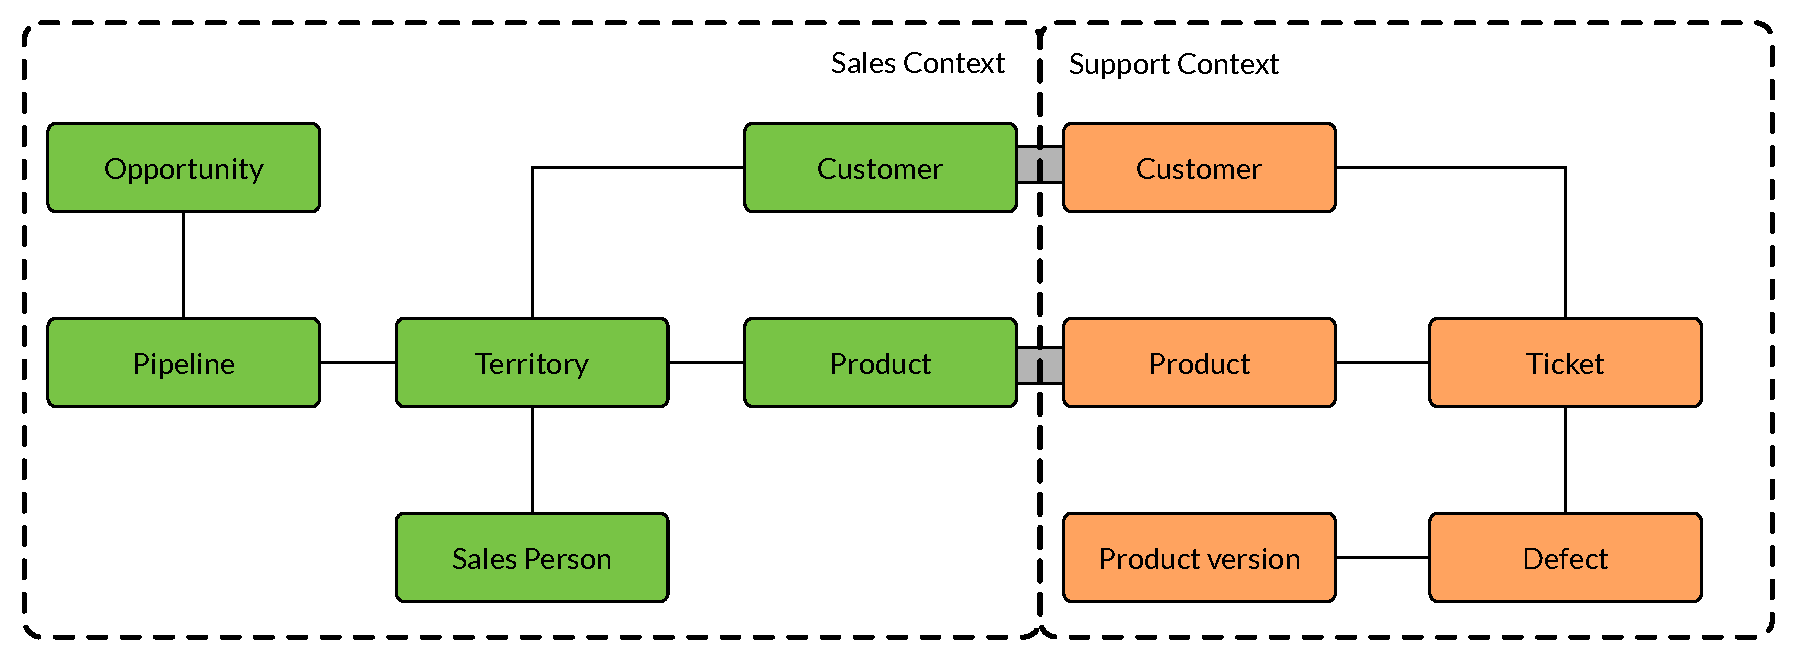
\includegraphics[width=\textwidth]{figures/bounded_context}
    \caption{Bounded Context \cite{boundedcontext2014fowler}}
    \label{fig:bounded_context}
\end{figure}

\noindent
The traditional way of managing large application is often, for management, to focus on separating into technology layers instead of business capabilities, leading to UI teams, server-side logic teams, and database teams. The problems that may arise when teams are separated along technology lines is that even simple changes can lead to cross team projects, resulting in longer implementation times. Melwyn Conway described in 1968 that an organization's communication structure will be reflected in the way teams design their systems. 

\begin{citat} []
"[...] organizations which design  systems (in the broad sense used here) are constrained to produce designs which are copies of the communication structures of these organizations" \textbf{- Melwyn Conway, 1968} \cite[p. 31]{conway1968law} 
\end{citat}


\noindent Figure~\ref{fig:conway} shows Conway's law in action. Siloed functional teams lead to siloed application architectures.
  

\begin{figure}[H]
    \centering
    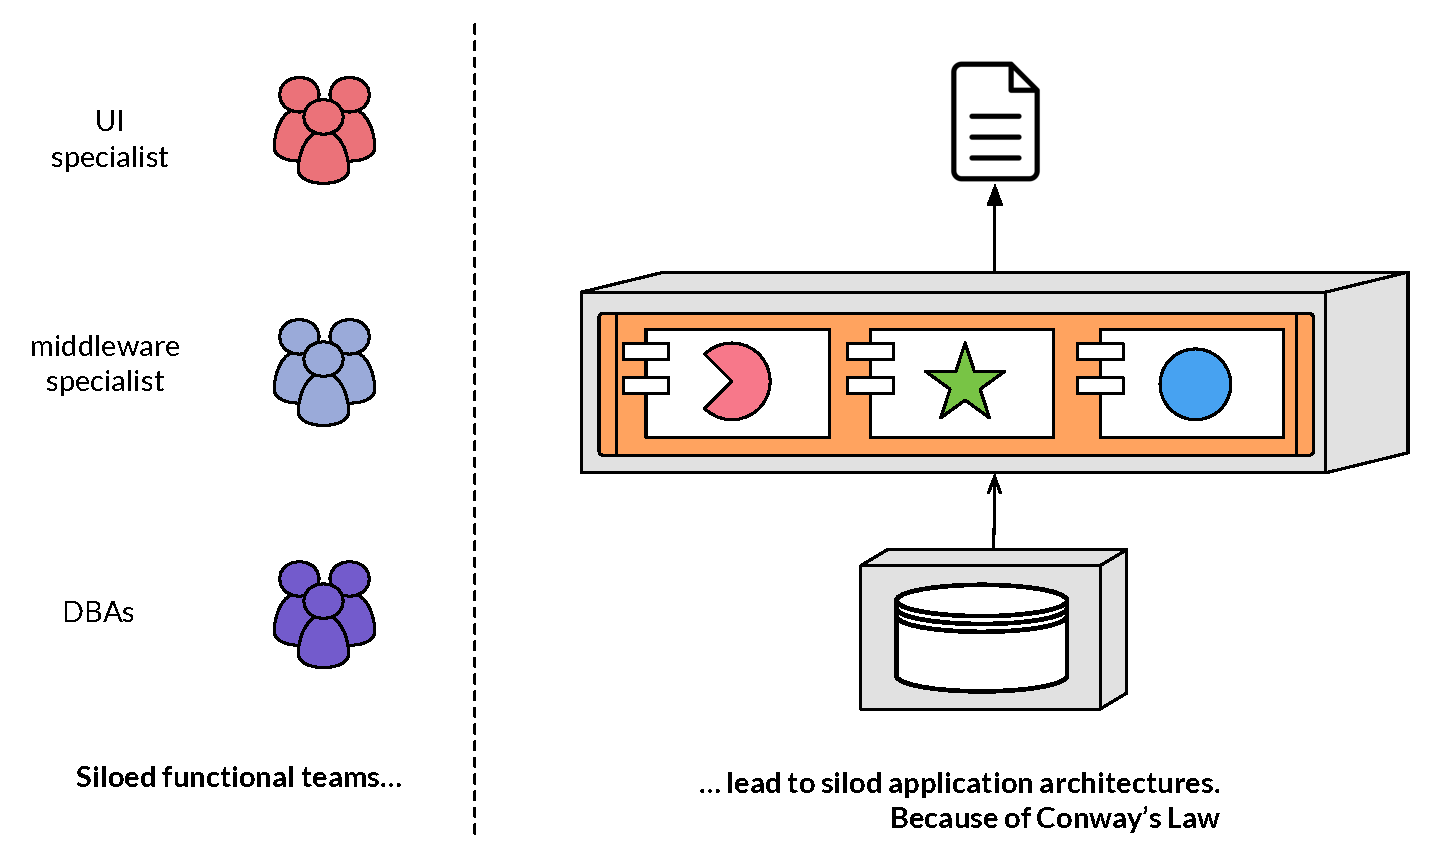
\includegraphics[width=12cm]{figures/conways_law}
    \caption{Conway's Law in Action \cite[p. 5]{lewis2014microservices}}
    \label{fig:conway}
\end{figure}


\noindent Instead, the microservice architectural approach is to organize around business capabilities in cross-functional and autonomous teams that clearly reinforce the boundaries between services and teams. Teams are responsible for the full stack, which is clearly reflected in Amazon's motto: \textit{"you build it, you run it"}. Newman describes this under his principle, \textit{Model Around Business Concepts}, and states that \textit{"interfaces structured around business-bounded contexts are more stable than those structured around technical concepts"} \cite[p. 246]{newman2015building}. The microservice approach to organization is depicted in Figure~\ref{fig:micro_business_capabilities}.

\begin{figure}[H]
    \centering
    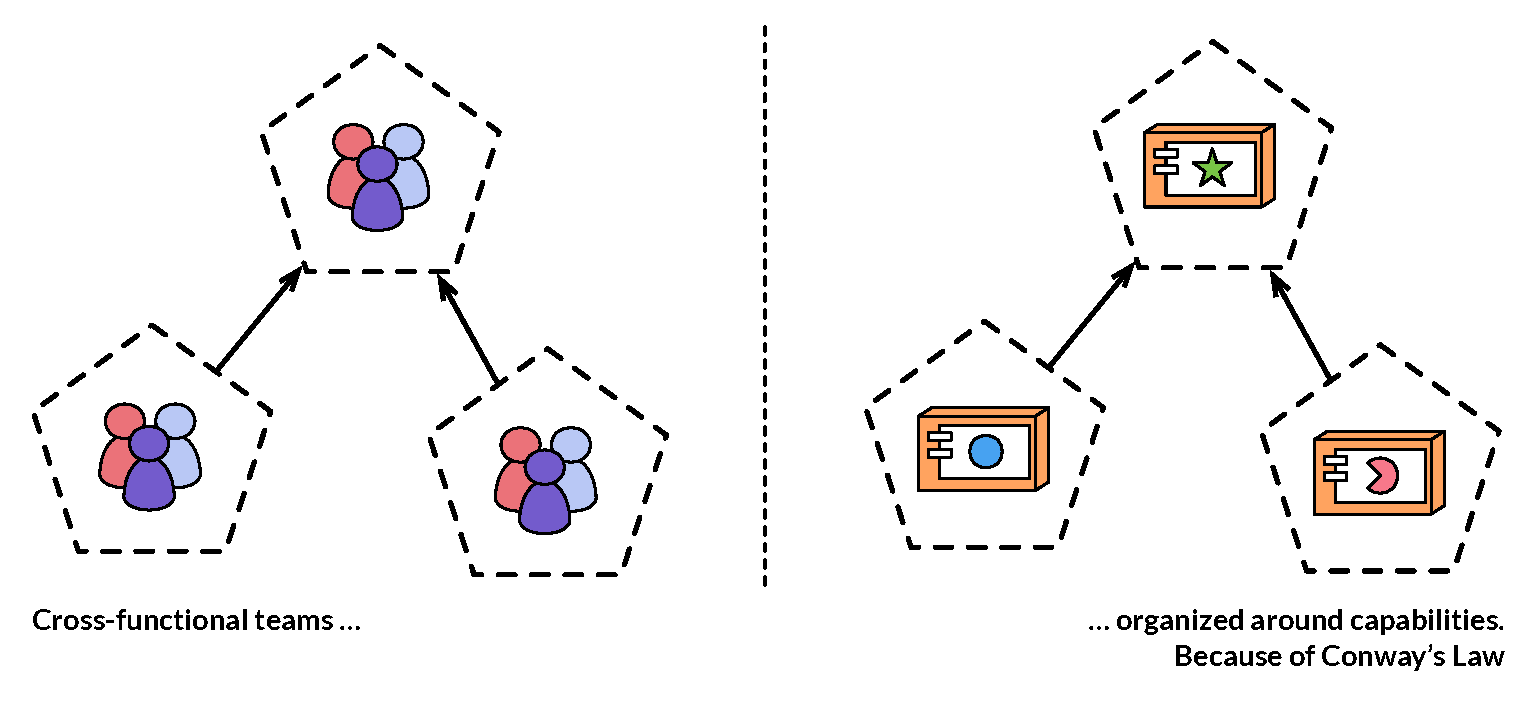
\includegraphics[width=\textwidth]{figures/microservices_capabilities}
    \caption{Organized around Business Capabilities \cite[p. 6]{lewis2014microservices}}
    \label{fig:micro_business_capabilities}
\end{figure}






\newpage
\noindent\textbf{Products not Projects} \\
Many application development efforts use a project model where the goal is to deliver software. When the software is developed and delivered, the project is considered complete. In many cases the software is then handed over to a maintenance or operations team and the project team, that build the software, is disbanded. Microservice architecture style tries to avoid this model, by preferring the notion that a team should own a product over its full lifetime. Rather than looking at software as a set of functionality to be completed, there is an on-going relationship where the question is: \textit{"how can software assist its users to enhance the business capability"} as Fowler and Lewis describe it \cite[p. 7]{lewis2014microservices}.\\

\noindent\textbf{Smart Endpoints and Dumb Pipes} \\
There exist multiple ways of communicating between different processes. One approach is the Enterprise Service Bus (ESB) which puts a lot of \textit{smarts} into the middleware layer. The Enterprise Service Bus is as mentioned in Chapter~\ref{chap:fundamentals_cloud_computing_architecture} an architecture used for designing and implementing communication between software applications in a service-oriented architecture (SOA). The ESB is responsible for e.g. routing of message exchanges between services and a lot other \textit{smarts}. The microservice community favors putting the smarts into the services instead of in the middleware. They build decoupled and highly cohesive services that own their own domain logic. The most commonly used protocols are HTTP and lightweight messaging, such as RabbitMQ or ZeroMQ. \\

\noindent\textbf{Decentralized Governance}\\
Fowler and Lewis state that \textit{"one of the consequences with centralized governance is the tendency to standardize on single technology platforms"} \cite[p. 7-8]{lewis2014microservices}. This approach is constricting  - \textit{"not every problem is a nail and not every solution is a hammer"} \cite[p. 8]{lewis2014microservices}. When splitting applications into services, architects have the choice of using the right tool for the particular responsibility, that a specific service needs to fulfil. The team is not restricted to use a specific technology, since they are working on an isolated service. However, \textit{"just because you can do something, doesn't mean you should"} \cite[p. 8]{lewis2014microservices}. The technology stack is not the only decentralized part in a microservice architecture. Centralized standards are not preferred and teams usually build helpful tools instead that can be shared among teams and even open sourced. Newman describes decentralization in his seven principles in the principle \textit{Decentralize all the things}, where he describes the importance of \textit{"embracing self-service wherever possible, allowing people to deploy software on demand, making development and testing as easy as possible, and avoiding the need for separate teams to perform these activities"}. \cite[p. 247]{newman2015building} \\

\noindent\textbf{Decentralized Data Management} \\
The monolithic approach is having one central database. This method can introduce lots of difficulties, since we allow different services to view and bind to the internal implementation details of the database schema. All services using this shared database have access and basically, the database is shared in its entirety. If a service wants to change the schema, represent the data better, or make the service easier to maintain, all services using the database will break. Furthermore, this approach ties consumers of the database to a specific technology choice. As Newman mentions, \textit{"perhaps right now it makes sense to store customers in a relational database [...] what if over time we realize we would be better off storing data in a nonrelational database?"}  \cite[p. 41]{newman2015building}. This approach has high coupling between services that consume the database and the database itself, which is not desirable. \\

\noindent
Instead of having one central database implementing the entire domain model, microservice architectures embrace the concept of decentralized data management. Again referring to the principles of Domain Driven Design and the notion of bounded contexts. This results in bounded contexts owning their own data and domain model and only exposing necessary data through its external interfaces. Fowler and Lewis describe that the microservice community  \textit{"prefers letting each service manage its own database, either as different instances of the same database technology or as entirely different database systems. This approach is called Polyglot Persistence"} \cite[p. 9]{lewis2014microservices}. Newman contributes to this view: \textit{"Services should hide their database to avoid falling into one of the most common sorts of coupling that can appear in traditional service-oriented architectures, and use data pumps or event data pumps to consolidate data across multiple services."} \cite[p. 247]{newman2015building}. Figure~\ref{fig:micro_decentralized_datamanagement} shows the difference between the centralized and decentralized data management approach.

\begin{figure}[H]
    \centering
    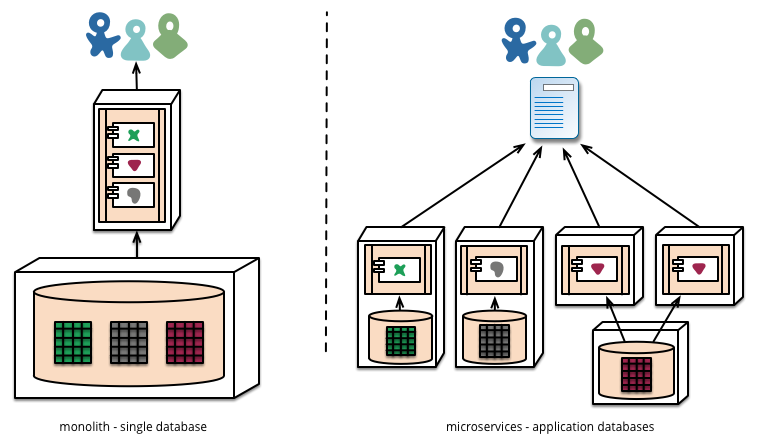
\includegraphics[width=\textwidth]{figures/microservice_decentralised-data}
    \caption{Decentralized Data Management \cite[p. 10]{lewis2014microservices}}
    \label{fig:micro_decentralized_datamanagement}
\end{figure}

\noindent Centralized data management is usually used within monolithic applications to ensure consistency. By using transactions in a centralized approach, it is easy to roll-back if something goes wrong. In the decentralized approach, distributed transactions are hard to implement, and working with microservices usually settles with eventual consistency. However the argument, as Fowler and Lewis state, \textit{"is that the trade-off of having to deal with a degree of inconsistency to respond quickly to demand is worth it if fixing mistakes is less than the cost of lost business under greater consistency."} \cite[p. 10]{lewis2014microservices} \\


\noindent\textbf{Infrastructure Automation} \\
One of the key enabling technologies for microservice architecture has been the evolution of infrastructure automation techniques for the past five years. This evolution has reduced the operational complexity of building, deploying and operating applications. Fowler and Lewis explain that \textit{"many of the products or systems being build with microservices are being built by teams with extensive knowledge of Continuous Delivery and its precursor Continuous Integration"}\cite[p. 10]{lewis2014microservices}. Two key concepts of Continuous Delivery worth mentioning are the extensive use of automated tests and the promotion of working software pipelines to automate deployments. Newman's \textit{Culture of Automation} principle describes this characteristic and states: \textit{"microservices add a lot of complexity, a key par of which comes from the sheer number of moving parts we have to deal with. Embracing a culture of automation is one key way to address this"} \cite[p. 246]{newman2015building}. He further states that \textit{"Automated testing is essential"}. When deploying monolithic applications the entire application usually has to be redeployed. Microservices allow teams to deploy services independently, making the deployment landscape strikingly different compared to monolithic applications. This is depicted in Figure~\ref{fig:micro-deployment}

\begin{figure}[H]
    \centering
    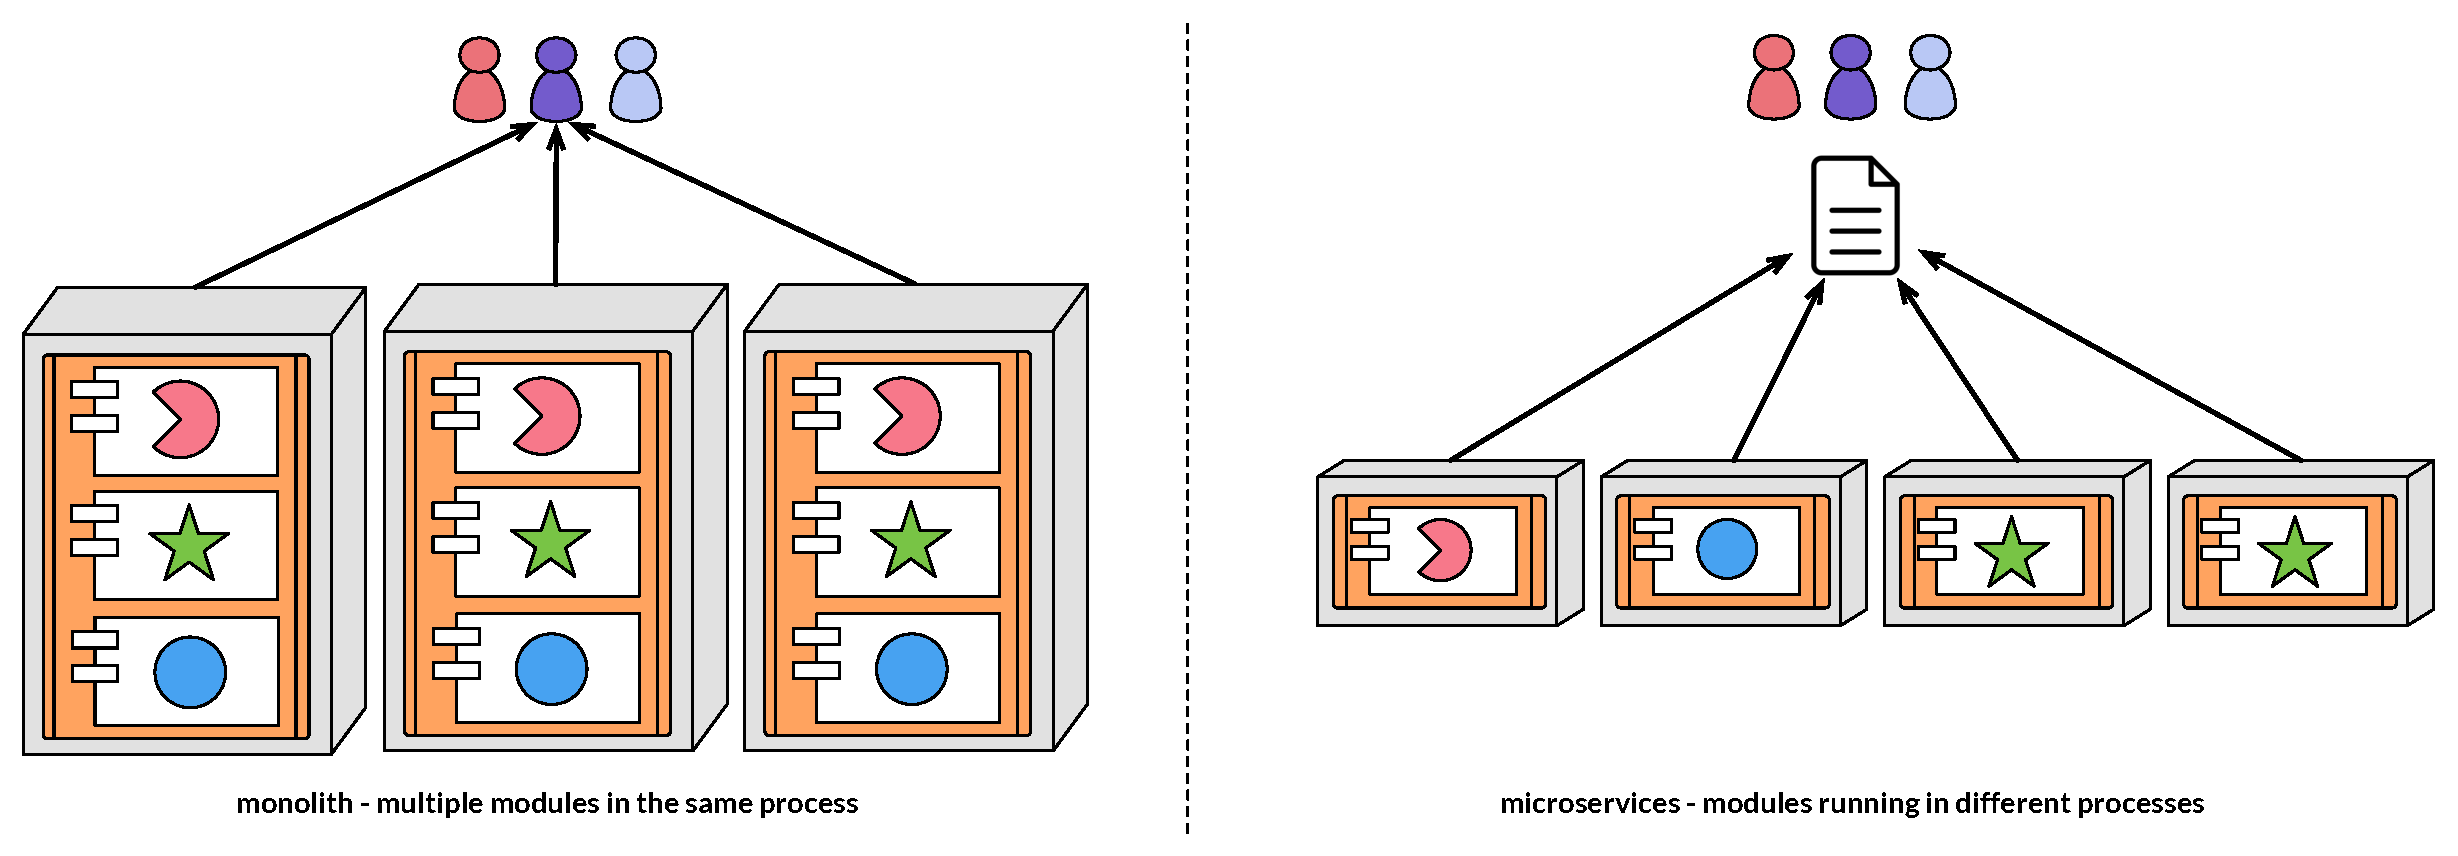
\includegraphics[width=\textwidth]{figures/micro-deployment}
    \caption{Infrastructure Automation \cite[p. 11]{lewis2014microservices}}
    \label{fig:micro-deployment}
\end{figure}

\noindent\textbf{Design for Failure} \\
One of the big consequences of transitioning from a monolithic architecture to a microservice architecture is the movement from an intra-process integrated application to a distributed modularized system. Any call between services can and will at some point fail, due to the non-deterministic behaviour of the underlying network. Microservice architecture therefore needs to be designed for failure, and to respond as gracefully as possible in case of failure. To cope with these potential failures, Netflix has introduced the Simian Army which is discussed in Chapter~\ref{chap_fundamentals_resilient_cloud}. Basically they introduce failures of services and even data centers during working days to test both applications' resilience and monitoring. Newman presents two principles that revolve around this characteristic, namely the principles Isolate failure and Highly observable. He states that \textit{"a microservice architecture can be more resilient than a monolithic system, but only if we understand and plan for failures in part of our system"} \cite[p. 248]{newman2015building}. Newman further emphasizes the importance of aggregation of logs and stats. \textit{We cannot rely on observing the behavior of a single service instance or the status of a single machine to see if the system is functioning correctly} \cite[p. 249]{newman2015building}. \\

\noindent\textbf{Evolutionary Design} \\
Fowler and Lewis state that \textit{"microservice practitioners come from an evolutionary design background and see service decomposition as a further tool to enable application developers to control changes in their application without slowing down change"} \cite[p. 12]{lewis2014microservices}. Controlling change does not necessarily mean a reduction in how frequent changes are implemented. When decomposing applications into services we are faced with the decision of how to slice up the application. Fowler and Lewis emphasize that the key property here \textit{"is the notion of independent replacement and upgradability"} \cite[p. 12]{lewis2014microservices}.

